\begin{figure}[H]
	\centering
	\begin{subfigure}[t]{0.45\linewidth}
		\centering
		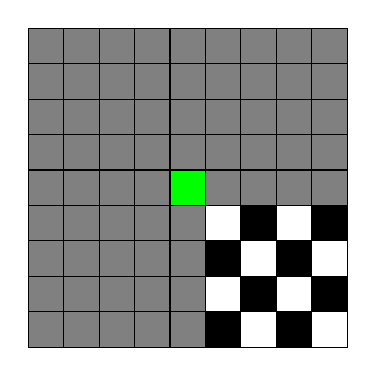
\begin{tikzpicture}[scale=0.45]
			\foreach \i in {-4, ..., 4}
				\foreach \j in {-4, ..., 4}
					\filldraw[gray] (\i, \j) rectangle + (1, 1);
			\foreach \i in {1, ..., 4}
				\foreach \j in {-4, ..., -1}
				{
					\pgfmathparse{mod(\i+\j, 2) ? "black" : "white"}
					\edef\colour{\pgfmathresult}
					\filldraw[fill=\colour] (\i, \j) rectangle + (1, 1);
				}
			\filldraw[green] (0, 0) rectangle + (1, 1);
			\draw[step=1] (-4, -4) grid (5, 5);
		\end{tikzpicture}
		\caption{Background pixel at the corner of the rROI.}
		\label{fig: background_corner}
	\end{subfigure}
	\hfill
	\begin{subfigure}[t]{0.45\linewidth}
		\centering
		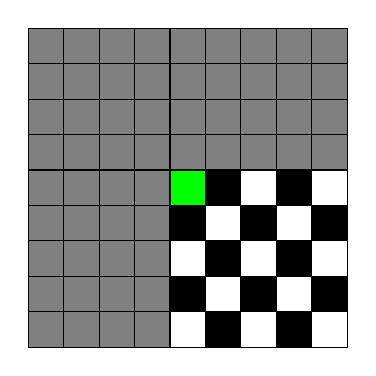
\begin{tikzpicture}[scale=0.45]
			\foreach \i in {-4, ..., 4}
				\foreach \j in {-4, ..., 4}
					\filldraw[gray] (\i, \j) rectangle + (1, 1);
			\foreach \i in {0, ..., 4}
				\foreach \j in {-4, ..., 0}
				{
					\pgfmathparse{mod(\i+\j, 2) ? "black" : "white"}
					\edef\colour{\pgfmathresult}
					\filldraw[fill=\colour] (\i, \j) rectangle + (1, 1);
				}
			\filldraw[green] (0, 0) rectangle + (1, 1);
			\draw[step=1] (-4, -4) grid (5, 5);
		\end{tikzpicture}
		\caption{Foreground pixel at the corner of the rROI.}
		\label{fig: foreground_corner}
	\end{subfigure}
	\vfill
	\begin{subfigure}[t]{0.45\linewidth}
		\centering
		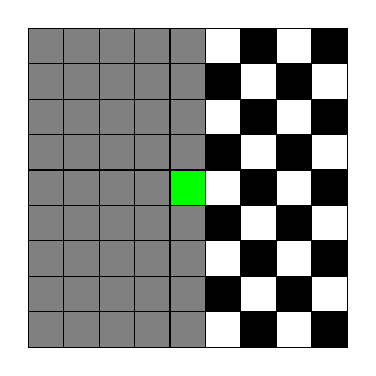
\begin{tikzpicture}[scale=0.45]
			\foreach \i in {-4, ..., 4}
				\foreach \j in {-4, ..., 4}
					\filldraw[gray] (\i, \j) rectangle + (1, 1);
			\foreach \i in {1, ..., 4}
				\foreach \j in {-4, ..., 4}
				{
					\pgfmathparse{mod(\i+\j+1, 2) ? "black" : "white"}
					\edef\colour{\pgfmathresult}
					\filldraw[fill=\colour] (\i, \j) rectangle + (1, 1);
				}
			\filldraw[green] (0, 0) rectangle + (1, 1);
			\draw[step=1] (-4, -4) grid (5, 5);
		\end{tikzpicture}
		\caption{Background pixel at the edge of the rROI.}
		\label{fig: background_edge}
	\end{subfigure}
	\hfill
	\begin{subfigure}[t]{0.45\linewidth}
		\centering
		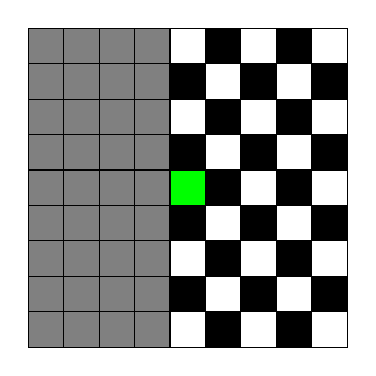
\begin{tikzpicture}[scale=0.45]
			\foreach \i in {-4, ..., 4}
				\foreach \j in {-4, ..., 4}
					\filldraw[gray] (\i, \j) rectangle + (1, 1);
			\foreach \i in {0, ..., 4}
				\foreach \j in {-4, ..., 4}
				{
					\pgfmathparse{mod(\i+\j, 2) ? "black" : "white"}
					\edef\colour{\pgfmathresult}
					\filldraw[fill=\colour] (\i, \j) rectangle + (1, 1);
				}
			\filldraw[green] (0, 0) rectangle + (1, 1);
			\draw[step=1] (-4, -4) grid (5, 5);
		\end{tikzpicture}
		\caption{Foreground pixel at the edge of the rROI.}
		\label{fig: foreground_edge}
	\end{subfigure}
	\vfill
	\begin{subfigure}[t]{0.45\linewidth}
		\centering
		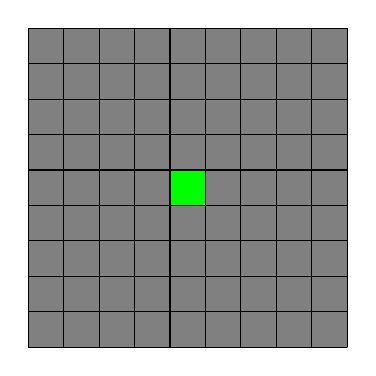
\begin{tikzpicture}[scale=0.45]
			\foreach \i in {-4, ..., 4}
				\foreach \j in {-4, ..., 4}
					\filldraw[gray] (\i, \j) rectangle + (1, 1);
			\filldraw[green] (0, 0) rectangle + (1, 1);
			\draw[step=1] (-4, -4) grid (5, 5);
		\end{tikzpicture}
		\caption{Background pixel surrounded by background.}
		\label{fig: background_free}
	\end{subfigure}
	\hfill
	\begin{subfigure}[t]{0.45\linewidth}
		\centering
		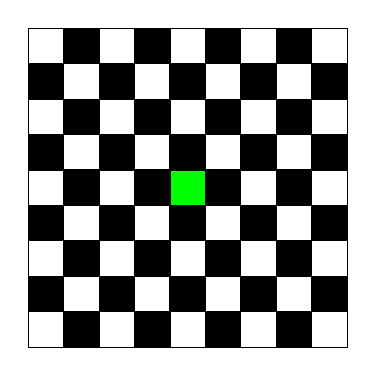
\begin{tikzpicture}[scale=0.45]
			\foreach \i in {-4, ..., 4}
				\foreach \j in {-4, ..., 4}
				{
					\pgfmathparse{mod(\i+\j, 2) ? "black" : "white"}
					\edef\colour{\pgfmathresult}
					\filldraw[fill=\colour] (\i, \j) rectangle + (1, 1);
				}
			\filldraw[green] (0, 0) rectangle + (1, 1);
			\draw[step=1] (-4, -4) grid (5, 5);
		\end{tikzpicture}
		\caption{Foreground pixel surrounded by foreground.}
		\label{fig: foreground_free}
	\end{subfigure}
	\caption{Position of the simulated pixels with respect to the rROI.}
	\label{fig: simulatedpixeltypes}
\end{figure}